\section{实验验证}

本章介绍实验部分。第一节为实验平台的软硬件配置;第二节介绍LLM与数据集的选取,以及实验组设置;第三节分析单步迭代执行时间预测误差;第四节针对基于开销感知的内存优化策略,进行吞吐率优化测试;第五节针对基于公平性的用户请求调度策略,进行实时性测试;第六节进行其它测试工作。

\subsection{实验环境}

本文开展实验使用的服务器软硬件配置如表\ref{Table:实验平台的软硬件配置}。

\begin{table}[H]
  \centering
  \caption{实验平台的软硬件配置}
  \label{Table:实验平台的软硬件配置}
  \renewcommand{\arraystretch}{1.2}
  \small
  \begin{tabular}{c c}
    \toprule
    \textbf{软件/硬件} & \textbf{型号/版本} \\ 
    \midrule
    CPU & Intel(R) Xeon(R) CPU @ 2.60GHz  \\ 
    GPU & NVIDIA A800 PCIE 80GB \\ 
    OS & CentOS Linux 7 (Core) \\ 
    CUDA & 11.8 \\ 
    pytorch & 2.0.1 \\ 
    ray & 2.7.1 \\
    vllm & 0.2.5 \\ 
    \bottomrule
  \end{tabular}
\end{table}

使用Intel(R) Xeon(R) CPU和NVIDIA A800 80GB GPU,CUDA版本为11.8。使用pytorch-2.0.l、ray-2.7.1以及vllm-0.2.5作为底层框架进行开发。 \par

服务器使用PCIe连接实现GPU-CPU通信。PCIe传输带宽在传输数据量不同时差异显著,表\ref{Table:PCIe双向传输带宽}列出了部分情况。在计算张量交换开销时,需要根据单次实际传输的数据量(一般是一个Block或其中的一部分)找到对应的传输带宽值。

\begin{table}[H]
  \centering
  \caption{PCIe双向传输带宽}
  \label{Table:PCIe双向传输带宽}
  \renewcommand{\arraystretch}{1.2}
  \small
  \begin{tabular}{c c c}
    \toprule
    \textbf{传输量(B)} & \textbf{HtoD(MB/s)} & \textbf{DtoH(MB/s)} \\
    \midrule
    1024 & 0.19 & 0.24 \\ 
    2048 & 0.60 & 0.72 \\ 
    4096 & 1.20 & 1.49 \\ 
    8192 & 1.07 & 2.97 \\ 
    16384 & 4.16 & 5.79 \\ 
    32768 & 7.76 & 9.35 \\ 
    102400 & 14.27 & 16.49 \\ 
    204800 & 18.30 & 20.24 \\ 
    409600 & 21.17 & 22.57 \\ 
    \bottomrule
  \end{tabular}
\end{table}

\subsection{实验设置}

本文选用OPT-13B、OPT-30B、Llama-13B和Llama-32.5B作为实验模型,在三个常见数据集上进行测试,如表\ref{Table:实验数据集选取}所示。

\begin{table}[H]
  \centering
  \caption{实验数据集选取}
  \label{Table:实验数据集选取}
  \renewcommand{\arraystretch}{1.2}
  \small
  \begin{tabular}{c c c c}
    \toprule
    \textbf{数据集} & \textbf{样本总数} & \textbf{平均输入长度} & \textbf{任务类型} \\
    \midrule
    chatbot & 258064 & 17.02 & 对话类 \\
    alpaca & 68912 & 19.66 & 指令类 \\
    summary & 1799 & 340.48 & 摘要类 \\
    \bottomrule
  \end{tabular}
\end{table}

三个数据集的样本序列长度分布曲线如图\ref{Fig:序列长度分布曲线}所示。chatbot和alpaca中大多数序列长度较短,而summary中序列长度展现出很大差异性,且包含长序列。它们涵盖了LLM应用程序面临的绝大部分场景。

\begin{figure}[!ht]
  \centering
  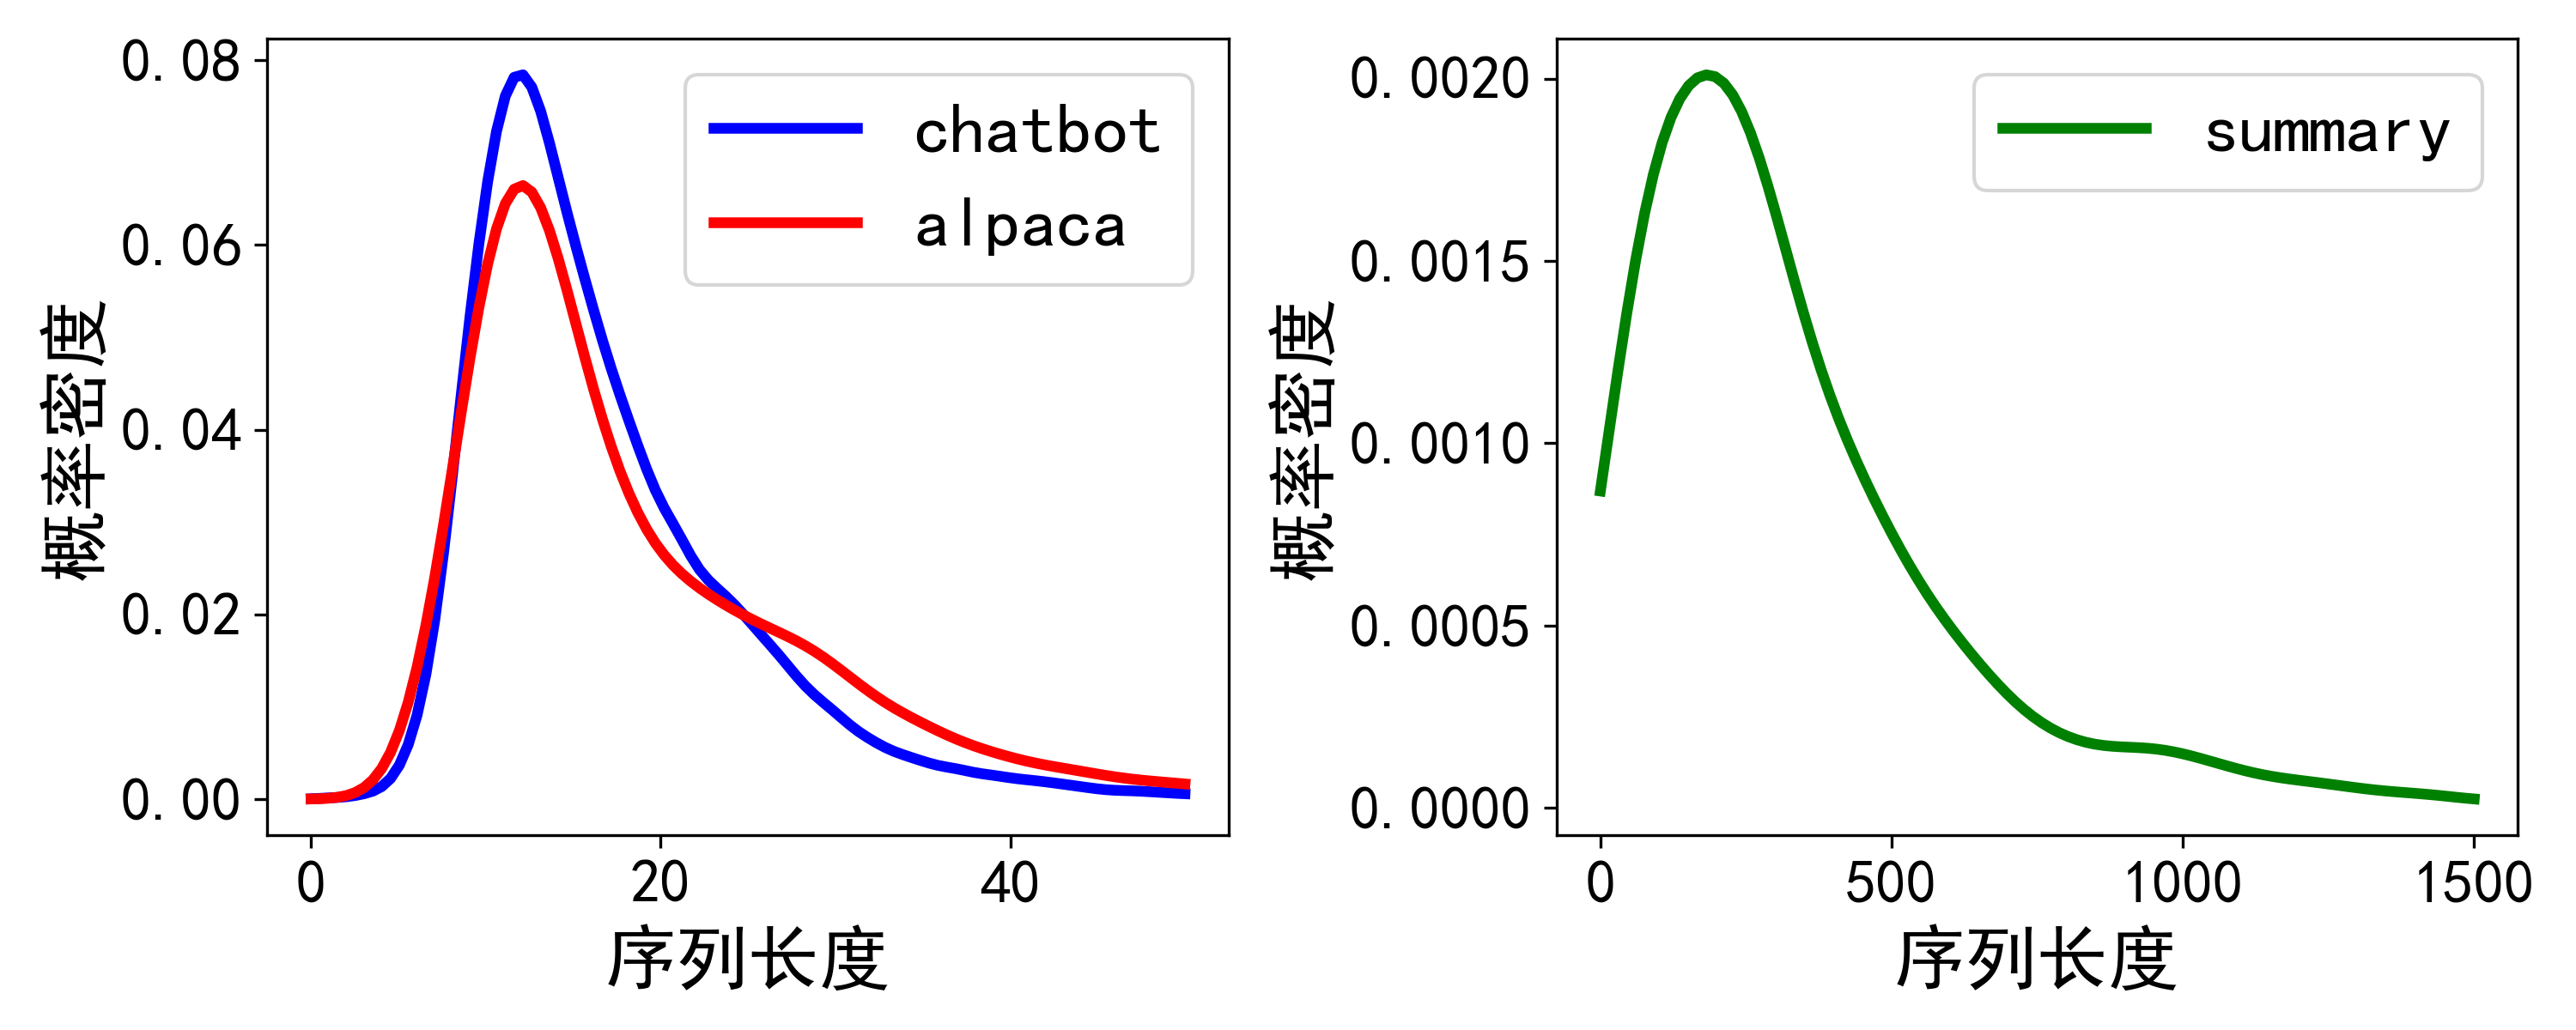
\includegraphics[width=0.9\linewidth]
  {序列长度分布曲线.png}
  \caption{序列长度分布曲线}
  \label{Fig:序列长度分布曲线}
\end{figure}

实验过程中的参数设置模拟LLM应用程序在多任务并发场景下的运行状态。本文将GPU Block数量设置为128,以保证推理任务执行过程中会发生抢占现象;将CPU Block数量设置为64,以保证张量重算技术能够在CPU内存不足时被调用。针对12个实验组,在相应数据集中使用简单随机抽样法选取1000个样本进行后续测试。

\subsection{执行时间预测}

表\ref{Table:OPT模型单步迭代执行时间预测误差}和表\ref{Table:LLama模型单步迭代执行时间预测误差}分别展示了OPT模型和Llama模型单步推理执行时间的预测效果。OPT执行时间预测任务共有6.4w条训练数据和1.6w条测试数据,结果表明,随机森林回归模型性能最佳,其在拟合2次多项式时能够达到1.76\%的预测误差。

\begin{table}[H]
  \centering
  \caption{OPT模型单步迭代执行时间预测误差}
  \label{Table:OPT模型单步迭代执行时间预测误差}
  \renewcommand{\arraystretch}{1.25}
  \small
  \begin{tabular}{c c c c c c}
    \toprule
    \textbf{模型-拟合次数} & \textbf{1} & \textbf{2} & \textbf{3} & \textbf{4} & \textbf{5} \\
    \midrule
    线性回归模型 & 46.52 & 46.65 & 28.75 & 11.86 & 9.32 \\ 
    支持向量机 & 27.76 & 23.51 & 17.88 & 14.03 & 11.29 \\
    决策树 & 1.81 & 1.81 & 1.81 & 1.81 & 1.81 \\ 
    随机森林 & 1.77 & 1.76 & 1.77 & 1.77 & 1.78 \\ 
    岭回归模型 & 46.52 & 46.37 & 28.45 & 11.51 & 7.36 \\ 
    lasso回归模型 & 40.22 & 25.53 & 27.38 & 26.08 & 25.49 \\ 
    弹性回归模型 & 111.89 & 123.62 & 91.67 & 87.59 & 86.48 \\ 
    梯度提升模型 & 15.57 & 16.05 & 14.80 & 15.09 & 14.68 \\ 
    KNN回归模型 & 2.55 & 2.80 & 2.89 & 3.00 & 3.05 \\ 
    \bottomrule
  \end{tabular}
\end{table}

Llama执行时间预测任务共有6.8条训练数据和1.7w条测试数据,结果表明,随机森林模型同样性能最佳,其在拟合2次多项式时能够达到1.30\%的预测误差。

\begin{table}[H]
  \centering
  \caption{LLama模型单步迭代执行时间预测误差}
  \label{Table:LLama模型单步迭代执行时间预测误差}
  \renewcommand{\arraystretch}{1.25}
  \small
  \begin{tabular}{c c c c c c}
    \toprule
    \textbf{模型-拟合次数} & \textbf{1} & \textbf{2} & \textbf{3} & \textbf{4} & \textbf{5} \\
    \midrule
    线性回归模型 & 76.41 & 69.44 & 39.61 & 12.91 & 9.18 \\ 
    支持向量机 & 55.82 & 37.50 & 26.44 & 22.92 & 19.19 \\ 
    决策树 & 1.33 & 1.32 & 1.33 & 1.33 & 1.34 \\ 
    随机森林 & 1.31 & 1.30 & 1.31 & 1.31 & 1.31 \\ 
    岭回归模型 & 76.41 & 69.01 & 39.18 & 12.73 & 7.72 \\ 
    lasso回归模型 & 69.23 & 33.57 & 34.42 & 35.16 & 31.58  \\ 
    弹性回归模型 & 127.18 & 139.7 & 100.18 & 94.94 & 93.51  \\ 
    梯度提升模型 & 22.42 & 21.97 & 19.42 & 19.99 & 19.38  \\ 
    KNN回归模型 & 2.24 & 2.36 & 2.48 & 2.63 & 2.68 \\ 
    \bottomrule
  \end{tabular}
\end{table}

\subsection{重算与交换的开销对比}

本文对OPT-13B、OPT-30B、Llama-13B和Llama-32.5B进行开销对比测试,其结果如图\ref{Fig:交换与重算开销对比}所示。当序列长度较小时,交换开销小于重算开销;随着序列长度的增加,二者大小关系反转。原因如下:  \par

自注意力机制内核采用并行计算策略,每个线程只计算一个token的qkv张量及注意力值。随着token数量增多,并行执行的线程数量增加,线程间同步开销随之上升,而单线程计算量不变。因此张量重算开销随序列长度增加呈亚线性增长。而由公式\ref{Eq:Swap Overhead}、\ref{Eq:Block Mem}、\ref{Eq:KV Cache Mem}可知,张量交换开销与序列长度呈近似正比关系。因此,张量重算开销的增长速度小于张量交换开销。  \par

\begin{figure}[!htbp]
  \centering
  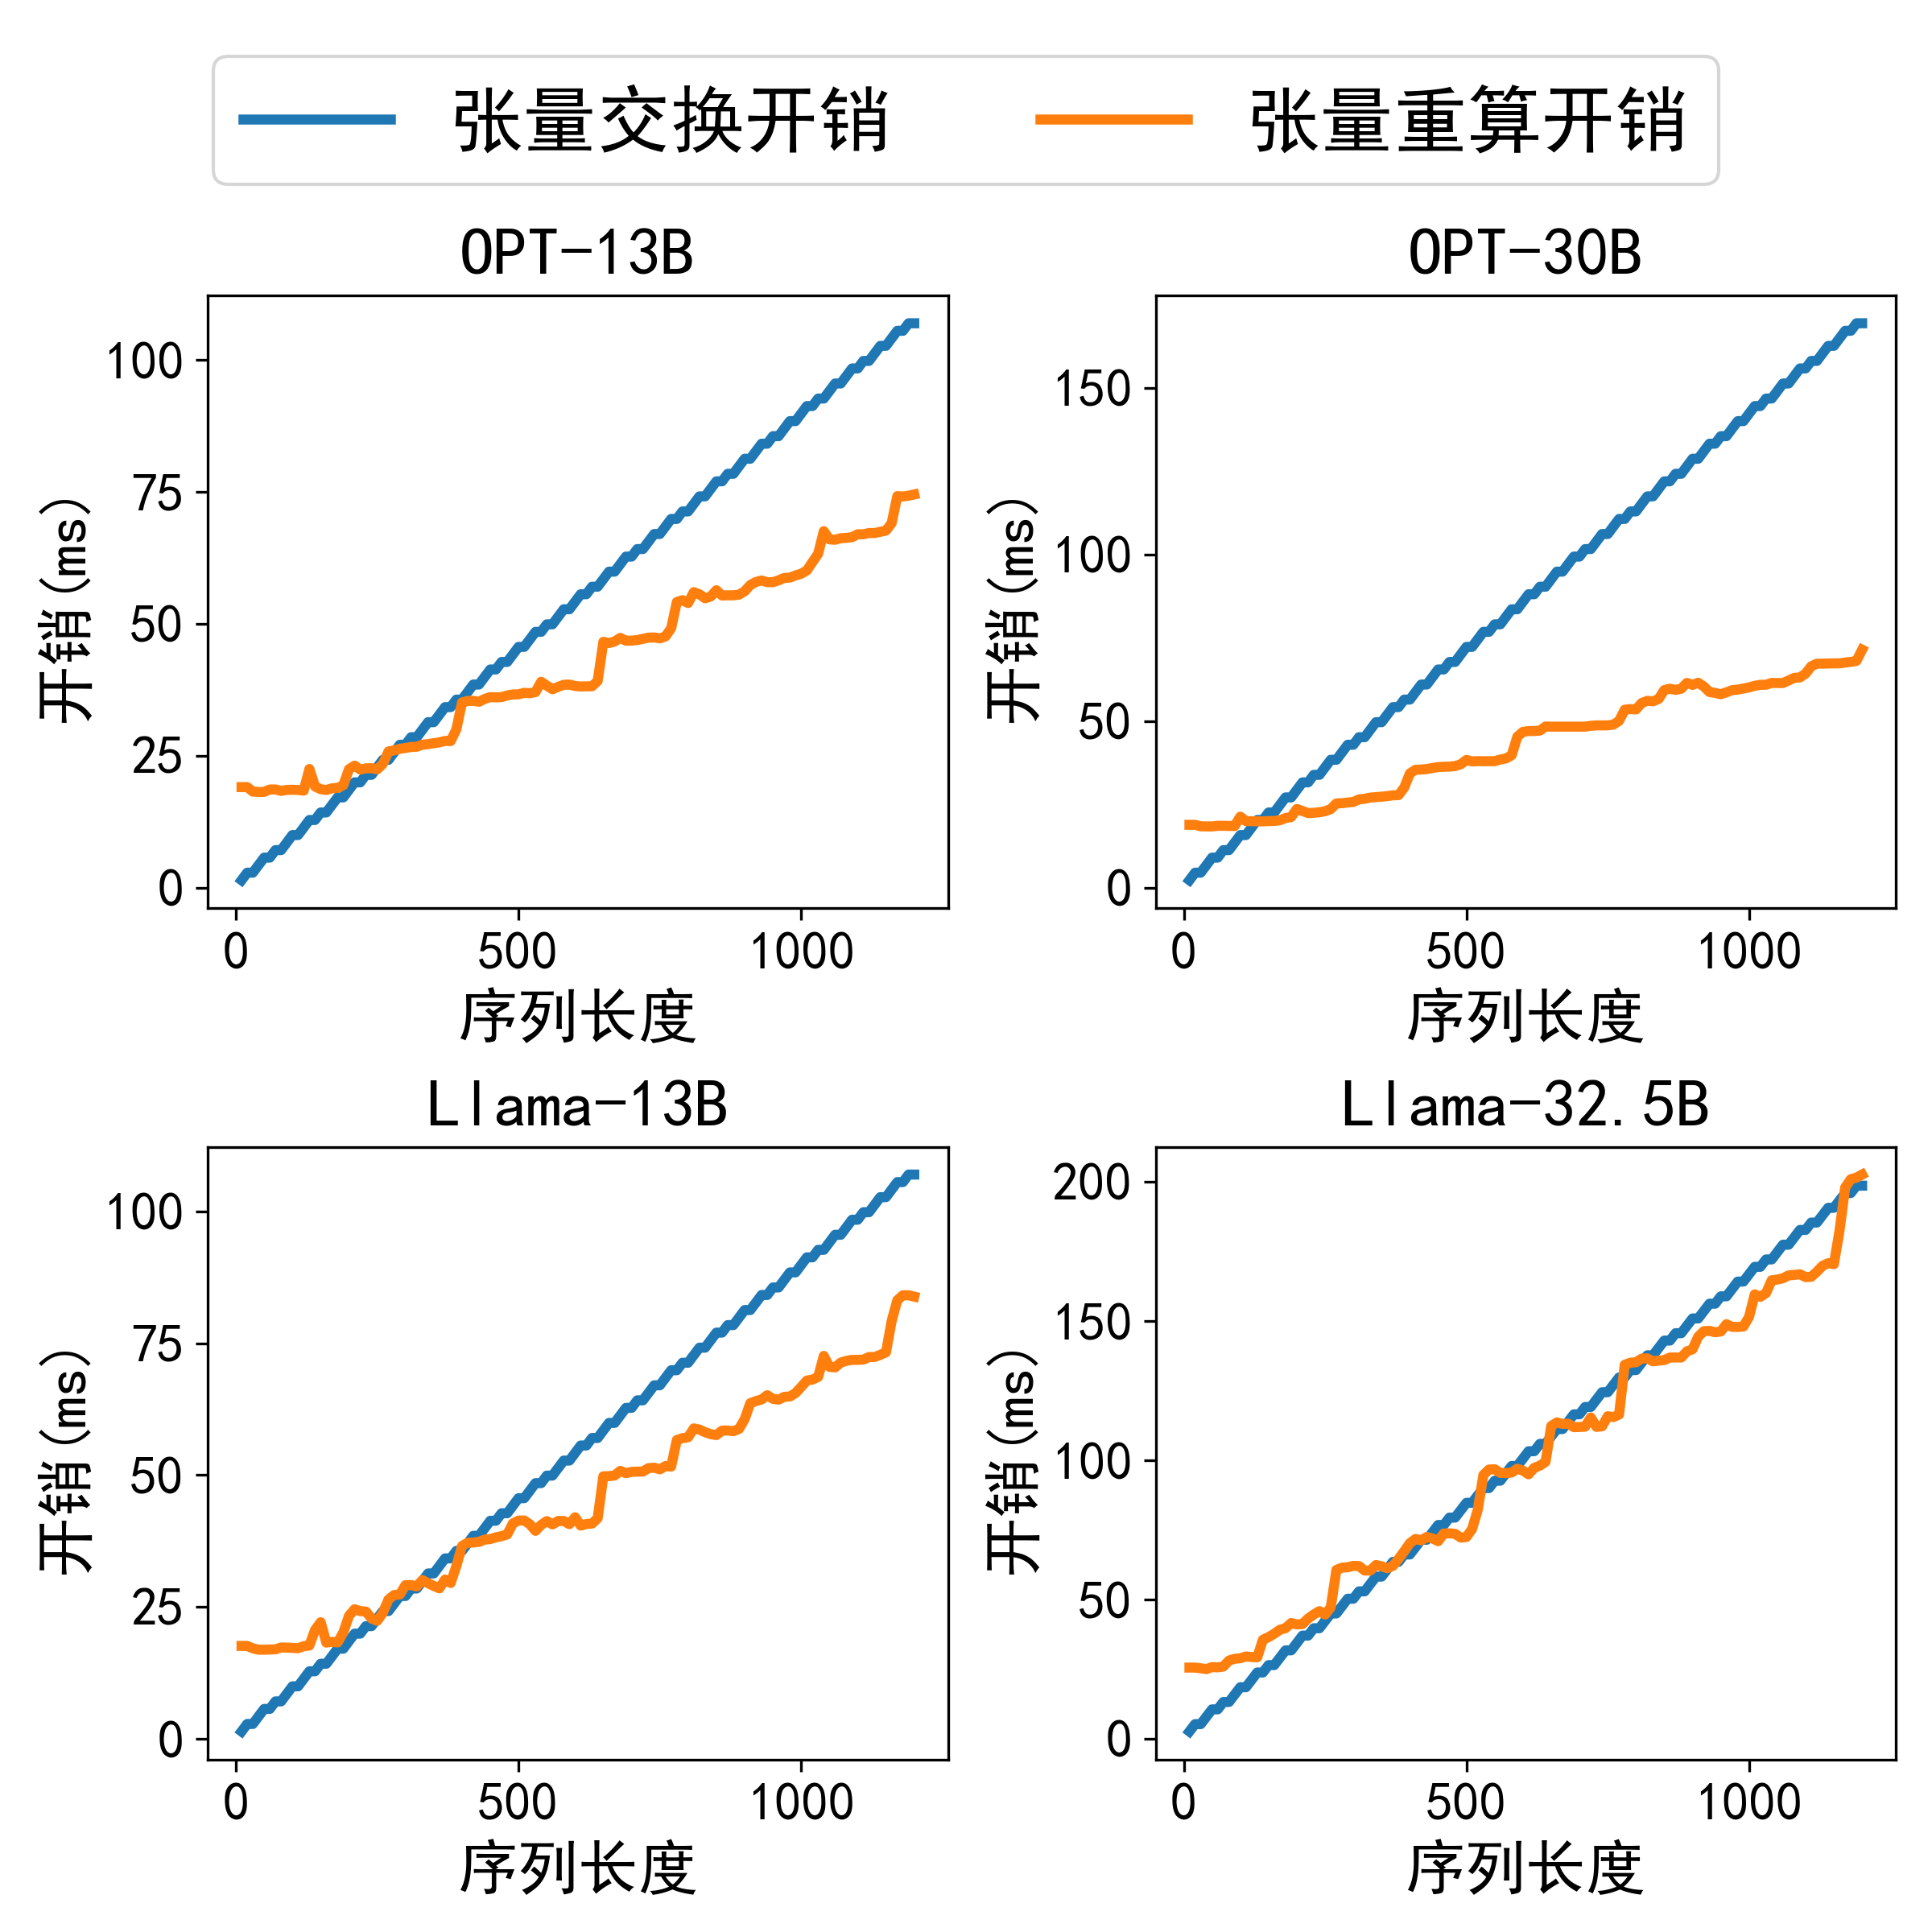
\includegraphics[width=0.9\linewidth]
  {交换与重算开销对比.png}
  \caption{交换与重算开销对比}
  \label{Fig:交换与重算开销对比}
\end{figure}

\begin{figure*}[!htbp]
  \centering
  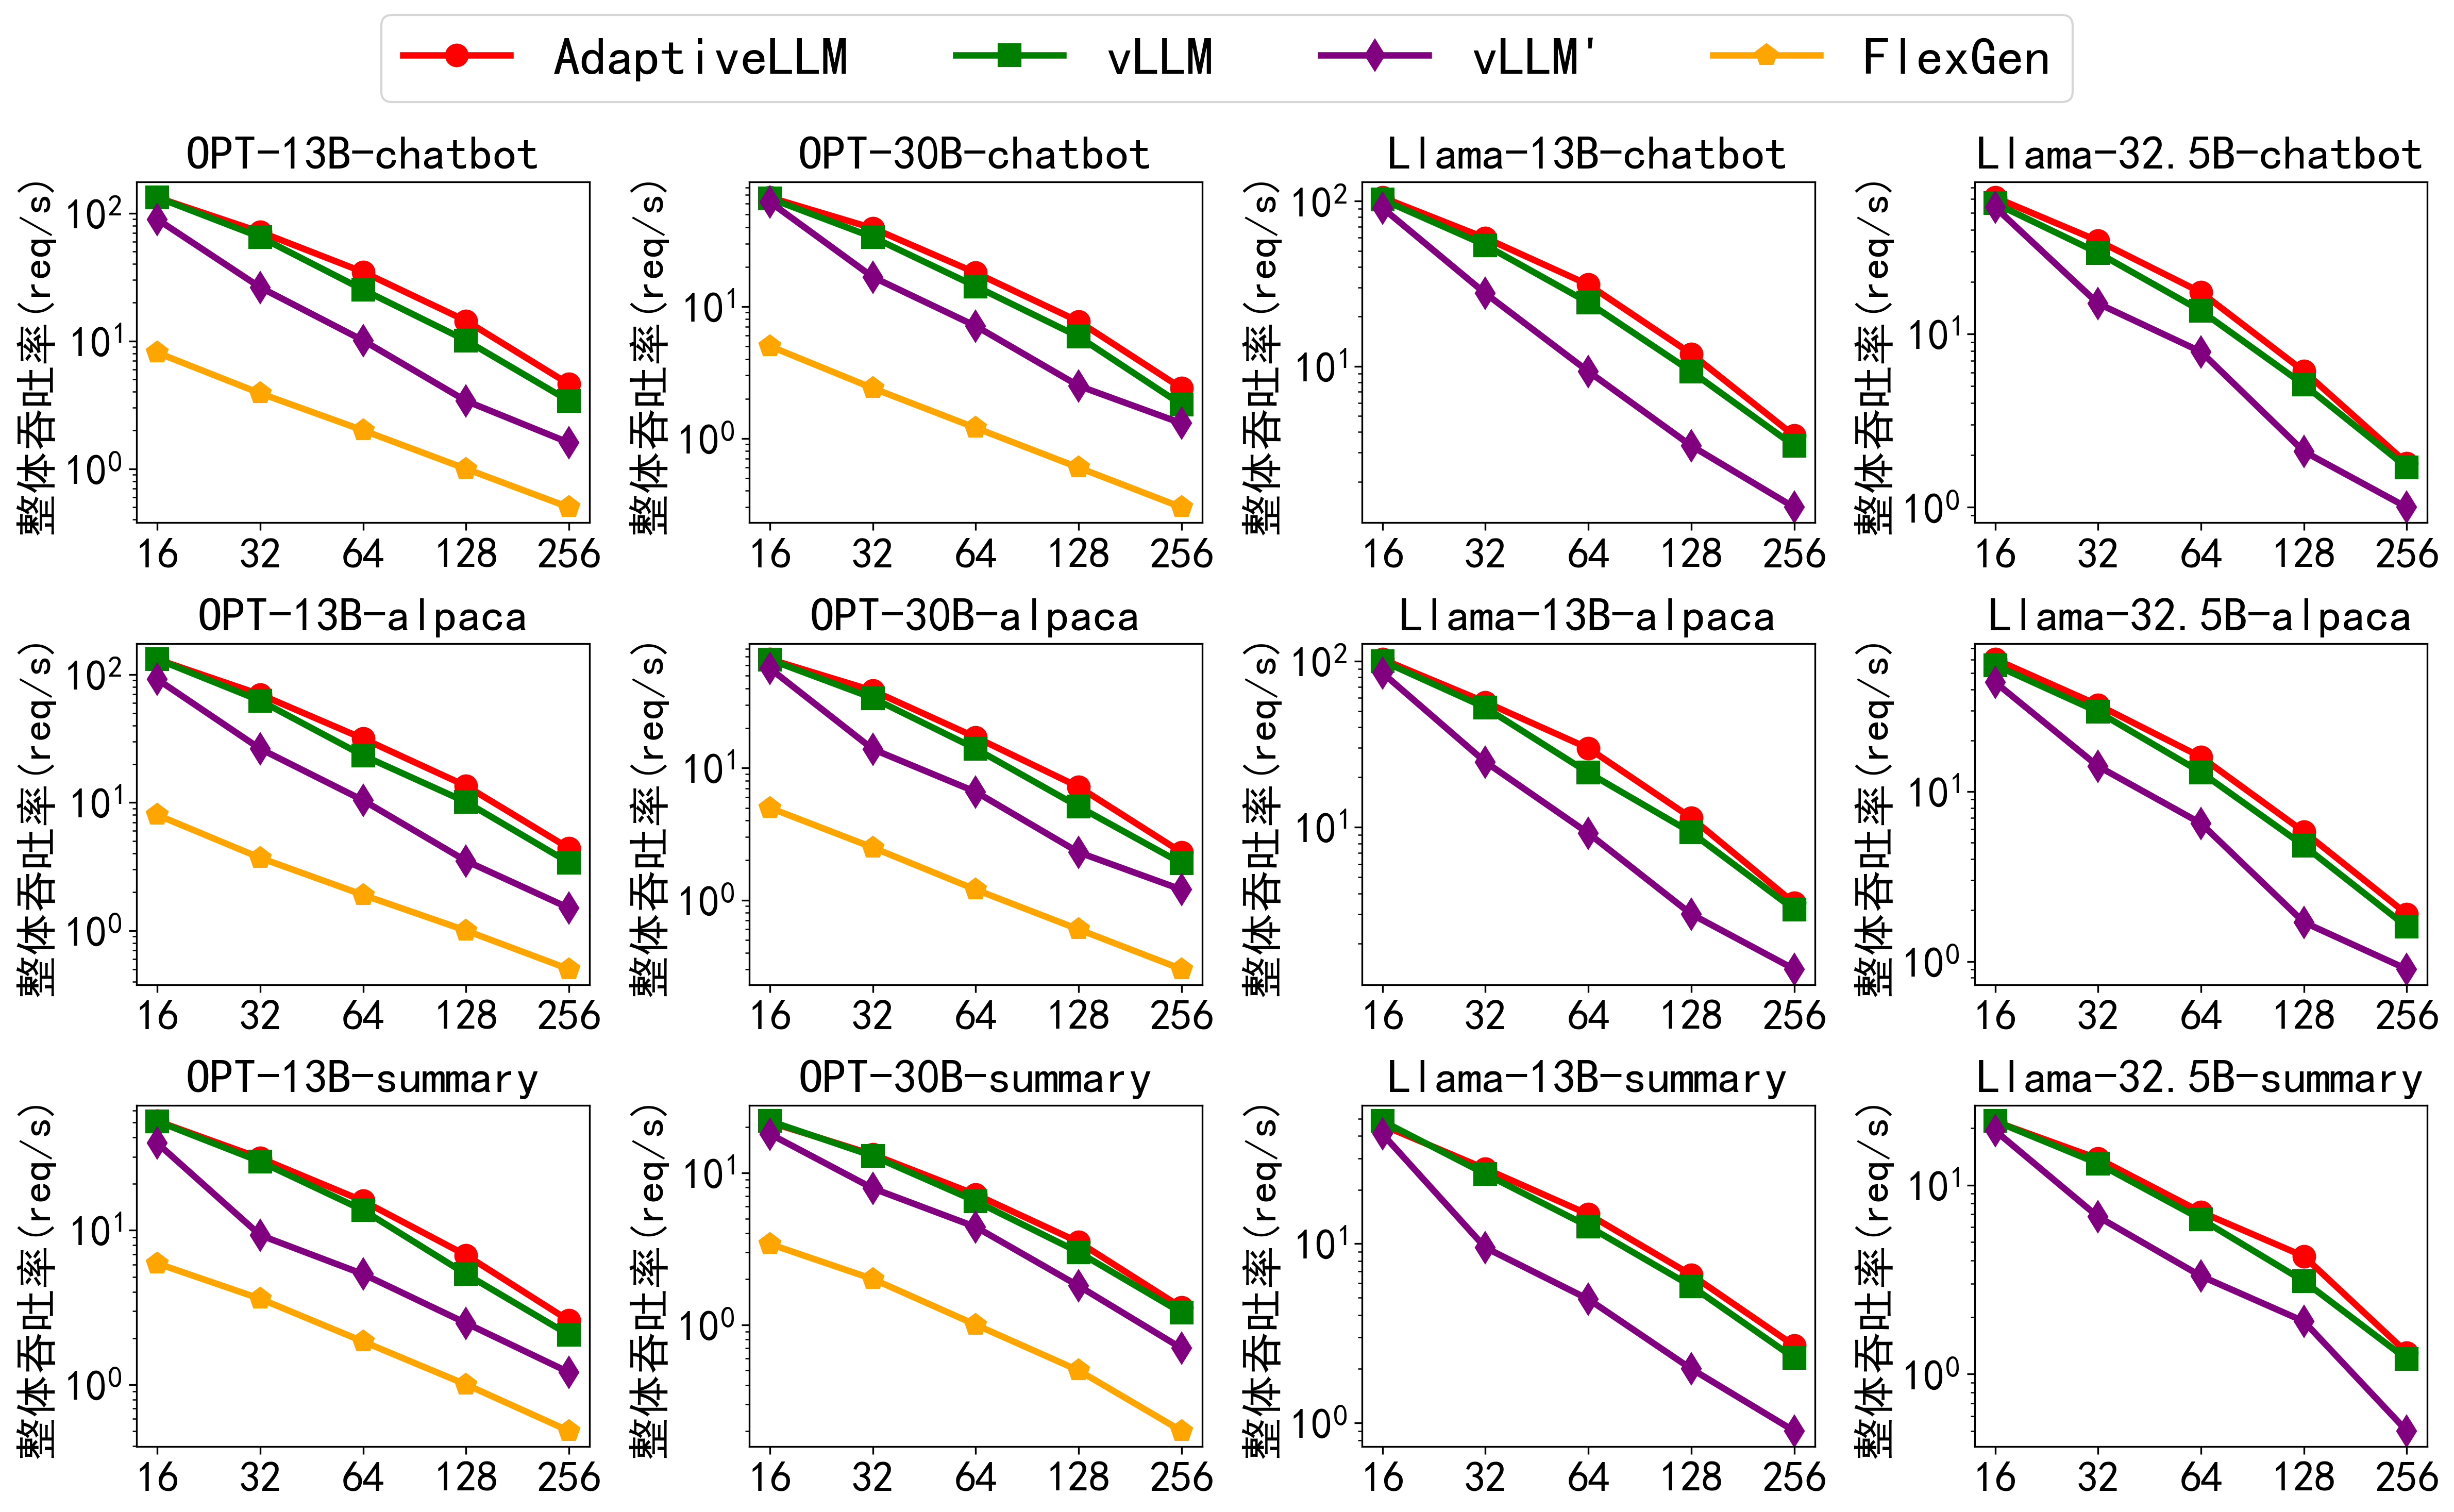
\includegraphics[width=0.85\linewidth]
  {推理任务吞吐率.png}
  \caption{推理任务吞吐率}
  \label{Fig:推理任务吞吐率}
\end{figure*}

在贪心采样策略下,对于长序列(如Summary数据集中的部分样本),无论是vLLM还是AdaptiveLLM,都偏向于使用重算,两种策略带来的抢占行为没有差异。对于短序列(如Chatbot和Alpaca数据集),vLLM使用重算,而AdaptiveLLM使用开销较小的交换,此时能够带来吞吐率提升。在LLM实际应用场景中,大多数序列的长度较短,使得张量交换在提升性能上拥有明显优势。而当长序列较多,或者CPU内存空间不足时,张量重算技术能够发挥优势。 

\subsection{吞吐率测试}

本文以vLLM作为基准框架,针对AdaptiveLLM进行吞吐率测试。同时,对vLLM框架稍加修改形成vLLM$\_$s,使得内存管理器在GPU内存不足时固定调用张量交换技术。 \par

图\ref{Fig:推理任务吞吐率}展示了12个实验组在推理任务中的整体吞吐率与序列最大输出长度的关系。表\ref{Table:AdaptiveLLM相对于vLLM的加速比}给出了最大输出长度为64时,AdaptiveLLM相对于vLLM的加速比。结果表明,以vLLM为基准框架时,基于开销感知的内存优化策略实现1.1到1.4的整体吞吐加速比。 \par

\begin{table}[H]
  \centering
  \caption{AdaptiveLLM相对于vLLM的加速比}
  \label{Table:AdaptiveLLM相对于vLLM的加速比}
  \renewcommand{\arraystretch}{1.25}
  \small
  \begin{tabular}{c c c c}
    \toprule
    \textbf{LLM-数据集} & \textbf{Chatbot} & \textbf{Alpaca} & \textbf{Summary} \\
    \midrule
    OPT-13B	& 1.377 & 1.356 & 1.148 \\
    OPT-30B	& 1.268 & 1.221 & 1.108 \\
    Llama-13B & 1.284 & 1.404 & 1.168 \\
    Llama-32.5B & 1.279 & 1.231 & 1.091 \\
    \bottomrule
  \end{tabular}
\end{table}

由于Summary数据集的平均序列长度和方差均明显高于Alpaca和Chatbot数据集,因此在相同条件下,其推理吞吐率低于Alpaca和Chatbot。同理,Alpaca在相同条件下的推理吞吐率应略低于Chatbot。

表\ref{Table:用户请求抢占行为记录}给出了序列最大输出长度为64时,不同框架推理过程中的抢占行为。 \par

\begin{table}[H]
  \centering
  \caption{用户请求抢占行为记录}
  \label{Table:用户请求抢占行为记录}
  \renewcommand{\arraystretch}{1.25}
  \small
  \begin{tabular}{c c c c c}
    \toprule
    \textbf{实验组} & \multicolumn{2}{c}{\textbf{AdaptiveLLM}} & \textbf{vLLM} & \textbf{vLLM$\_$s} \\
    \midrule
    \textbf{抢占行为(千次)} & \textbf{重算} & \textbf{交换} & \textbf{重算} & \textbf{交换} \\
    \midrule
    OPT-13B-chatbot & 0.11 & 1.13 & 1.77 & 0.78 \\
    OPT-13B-alpaca & 0.10 & 1.17 & 1.82 & 0.99 \\
    OPT-13B-summary & 0.10 & 0.56 & 0.58 & 0.26 \\
    OPT-30B-chatbot & 0.08 & 1.10 & 1.64 & 0.68 \\
    OPT-30B-alpaca & 0.10 & 1.05 & 1.61 & 0.59 \\
    OPT-30B-summary & 0.09 & 0.43 & 0.47 & 0.32 \\
    Llama-13B-chatbot & 0.12 & 1.02 & 1.57 & 0.83 \\
    Llama-13B-alpaca & 0.08 & 1.03 & 1.55 & 0.87 \\
    Llama-13B-summary & 0.15 & 0.55 & 0.57 & 0.36 \\
    Llama-32.5B-chatbot & 0.07 & 1.04 & 1.53 & 0.20 \\
    Llama-32.5B-alpaca & 0.10 & 1.00 & 1.57 & 0.55 \\
    \bottomrule
  \end{tabular}
\end{table}

在GPU内存不足时,vLLM调用张量重算技术;vLLM$\_$s调用张量交换技术;而AdaptiveLLM能够从二者中选择开销较小的抢占方式。CPU内存的限制使vLLM$\_$s的批处理大小低于vLLM和AdaptiveLLM,因此吞吐率也较低。当用户请求序列的最大输出长度限制在较低水平时,每个请求执行推理任务所需的迭代次数较少,资源需求量低,抢占鲜有发生,此时AdaptiveLLM和vLLM的性能差距不大。随着最大输出长度的增加,有限的GPU内存无法满足需求,AdaptiveLLM调用基于开销感知的内存优化策略,展现性能优势;当最大输出长度过大时,无论是AdaptiveLLM还是vLLM,其批处理大小均限制在较低水平,但AdaptiveLLM仍具有明显优势(当批处理大小为256时,AdaptiveLLM在vLLM的基础上实现了1.1到1.3的整体加速比)。\par

由表\ref{Table:用户请求抢占行为记录}可知,在Chatbot和Alpaca数据集的推理任务中,序列长度较短,批处理大小高,换出频繁,导致CPU内存不足,因此AdaptiveLLM执行了少量张量重算操作;在Summary数据集的推理任务中,其序列长度较大,批处理大小低,换入换出较少,极少出现CPU内存不足的现象,此时张量重算操作的执行大部分来源于开销比较的结果。 \par

另外,短序列被抢占时,张量交换相比于张量重算有开销优势。而OPT-13B和Llama-13B相比于OPT-30B和Llama-32.5B,这种优势更加明显,如图\ref{Fig:交换与重算开销对比}所示。因此在OPT-13B和Llama-13B上,AdaptiveLLM产生的加速比(以vLLM作为对照)更高。

\subsection{实时性测试}

为了消除整体吞吐率变化对实时性测试的影响,本文选取平均带权周转时间作为测试指标。用户请求带权周转时间等于客户端响应时间除以服务器端处理时间,如公式\ref{Eq:Weighted Around Time}所示。该指标越低,说明用户请求的排队时间越短。 \par

\begin{equation}
  \begin{aligned}
    w\_around\_t = \frac{finish\_t - send\_t}{finish\_t - sche\_t}
  \end{aligned}
  \label{Eq:Weighted Around Time}
  \setlength{\abovedisplayskip}{0ex}
  \setlength{\belowdisplayskip}{2ex}
\end{equation}

图\ref{Fig:用户请求平均带权周转时间}展示了平均带权周转时间随批处理大小上限的变化情况。在不同批处理大小设置下,基于公平性的用户请求调度策略均能使平均带权周转时间显著下降。当批处理大小较大时(64或128),AdaptiveLLM的平均带权周转时间为vLLM的60\%至80\%。

\begin{figure*}[!htbp]
  \centering
  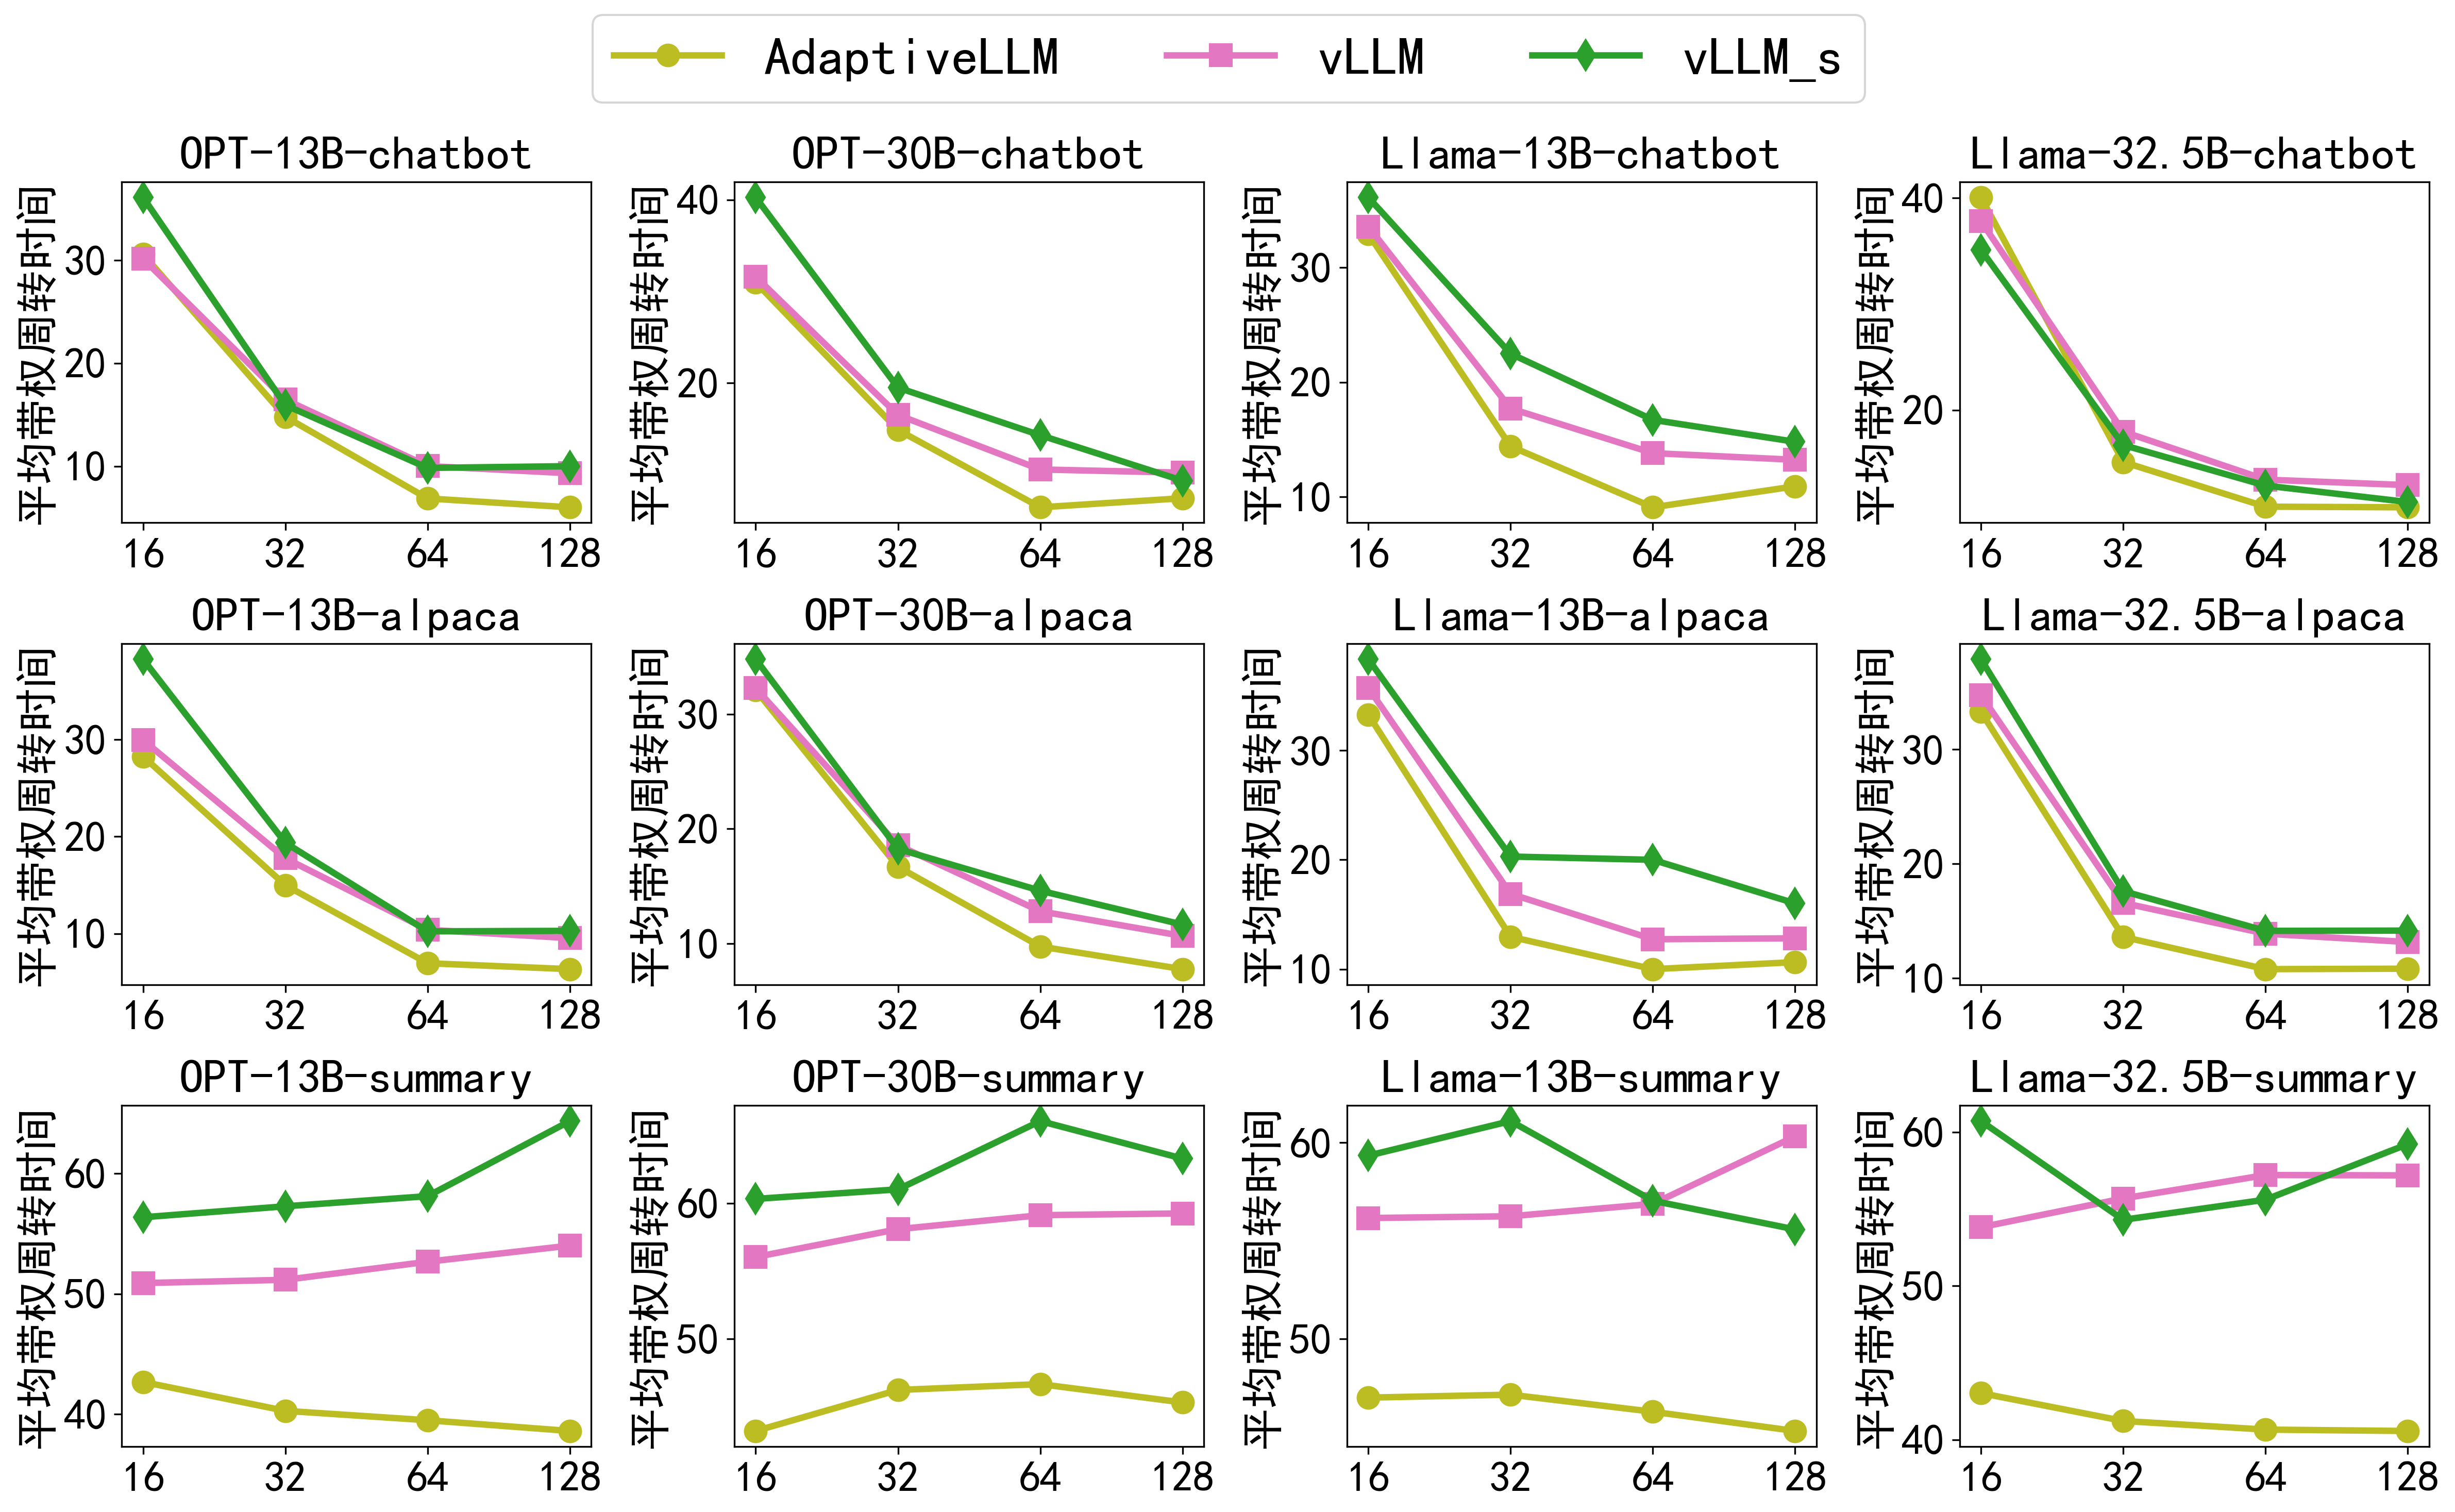
\includegraphics[width=0.85\linewidth]
  {用户请求平均带权周转时间.png}
  \caption{用户请求平均带权周转时间}
  \label{Fig:用户请求平均带权周转时间}
\end{figure*}

对于序列较短的Chatbot和Alpaca数据集而言,随着批处理大小的上升,GPU利用更加充分,因此平均带权周转时间下降。当批处理大小到达64时,GPU产生内存瓶颈,此时平均带权周转时间不再随最大批处理大小的上升而下降。 \par

对于序列较长的Summary数据集而言,其处理并发度被限制在较低水平(10以下),无法达到用户设置的批处理大小上限。因此平均带权周转时间呈稳定状态。AdaptiveLLM中高效的调度策略展现优势,使用户请求等待时间显著低于vLLM和vLLM\_s。\par

综上所述,基于公平性的用户请求调度策略使得用户请求从客户端发送至服务器端后能够很快开始处理,不会出现长时间等待现象。

\subsection{其它测试}

\subsubsection{误差分析}

\begin{figure}[!htbp]
  \centering
  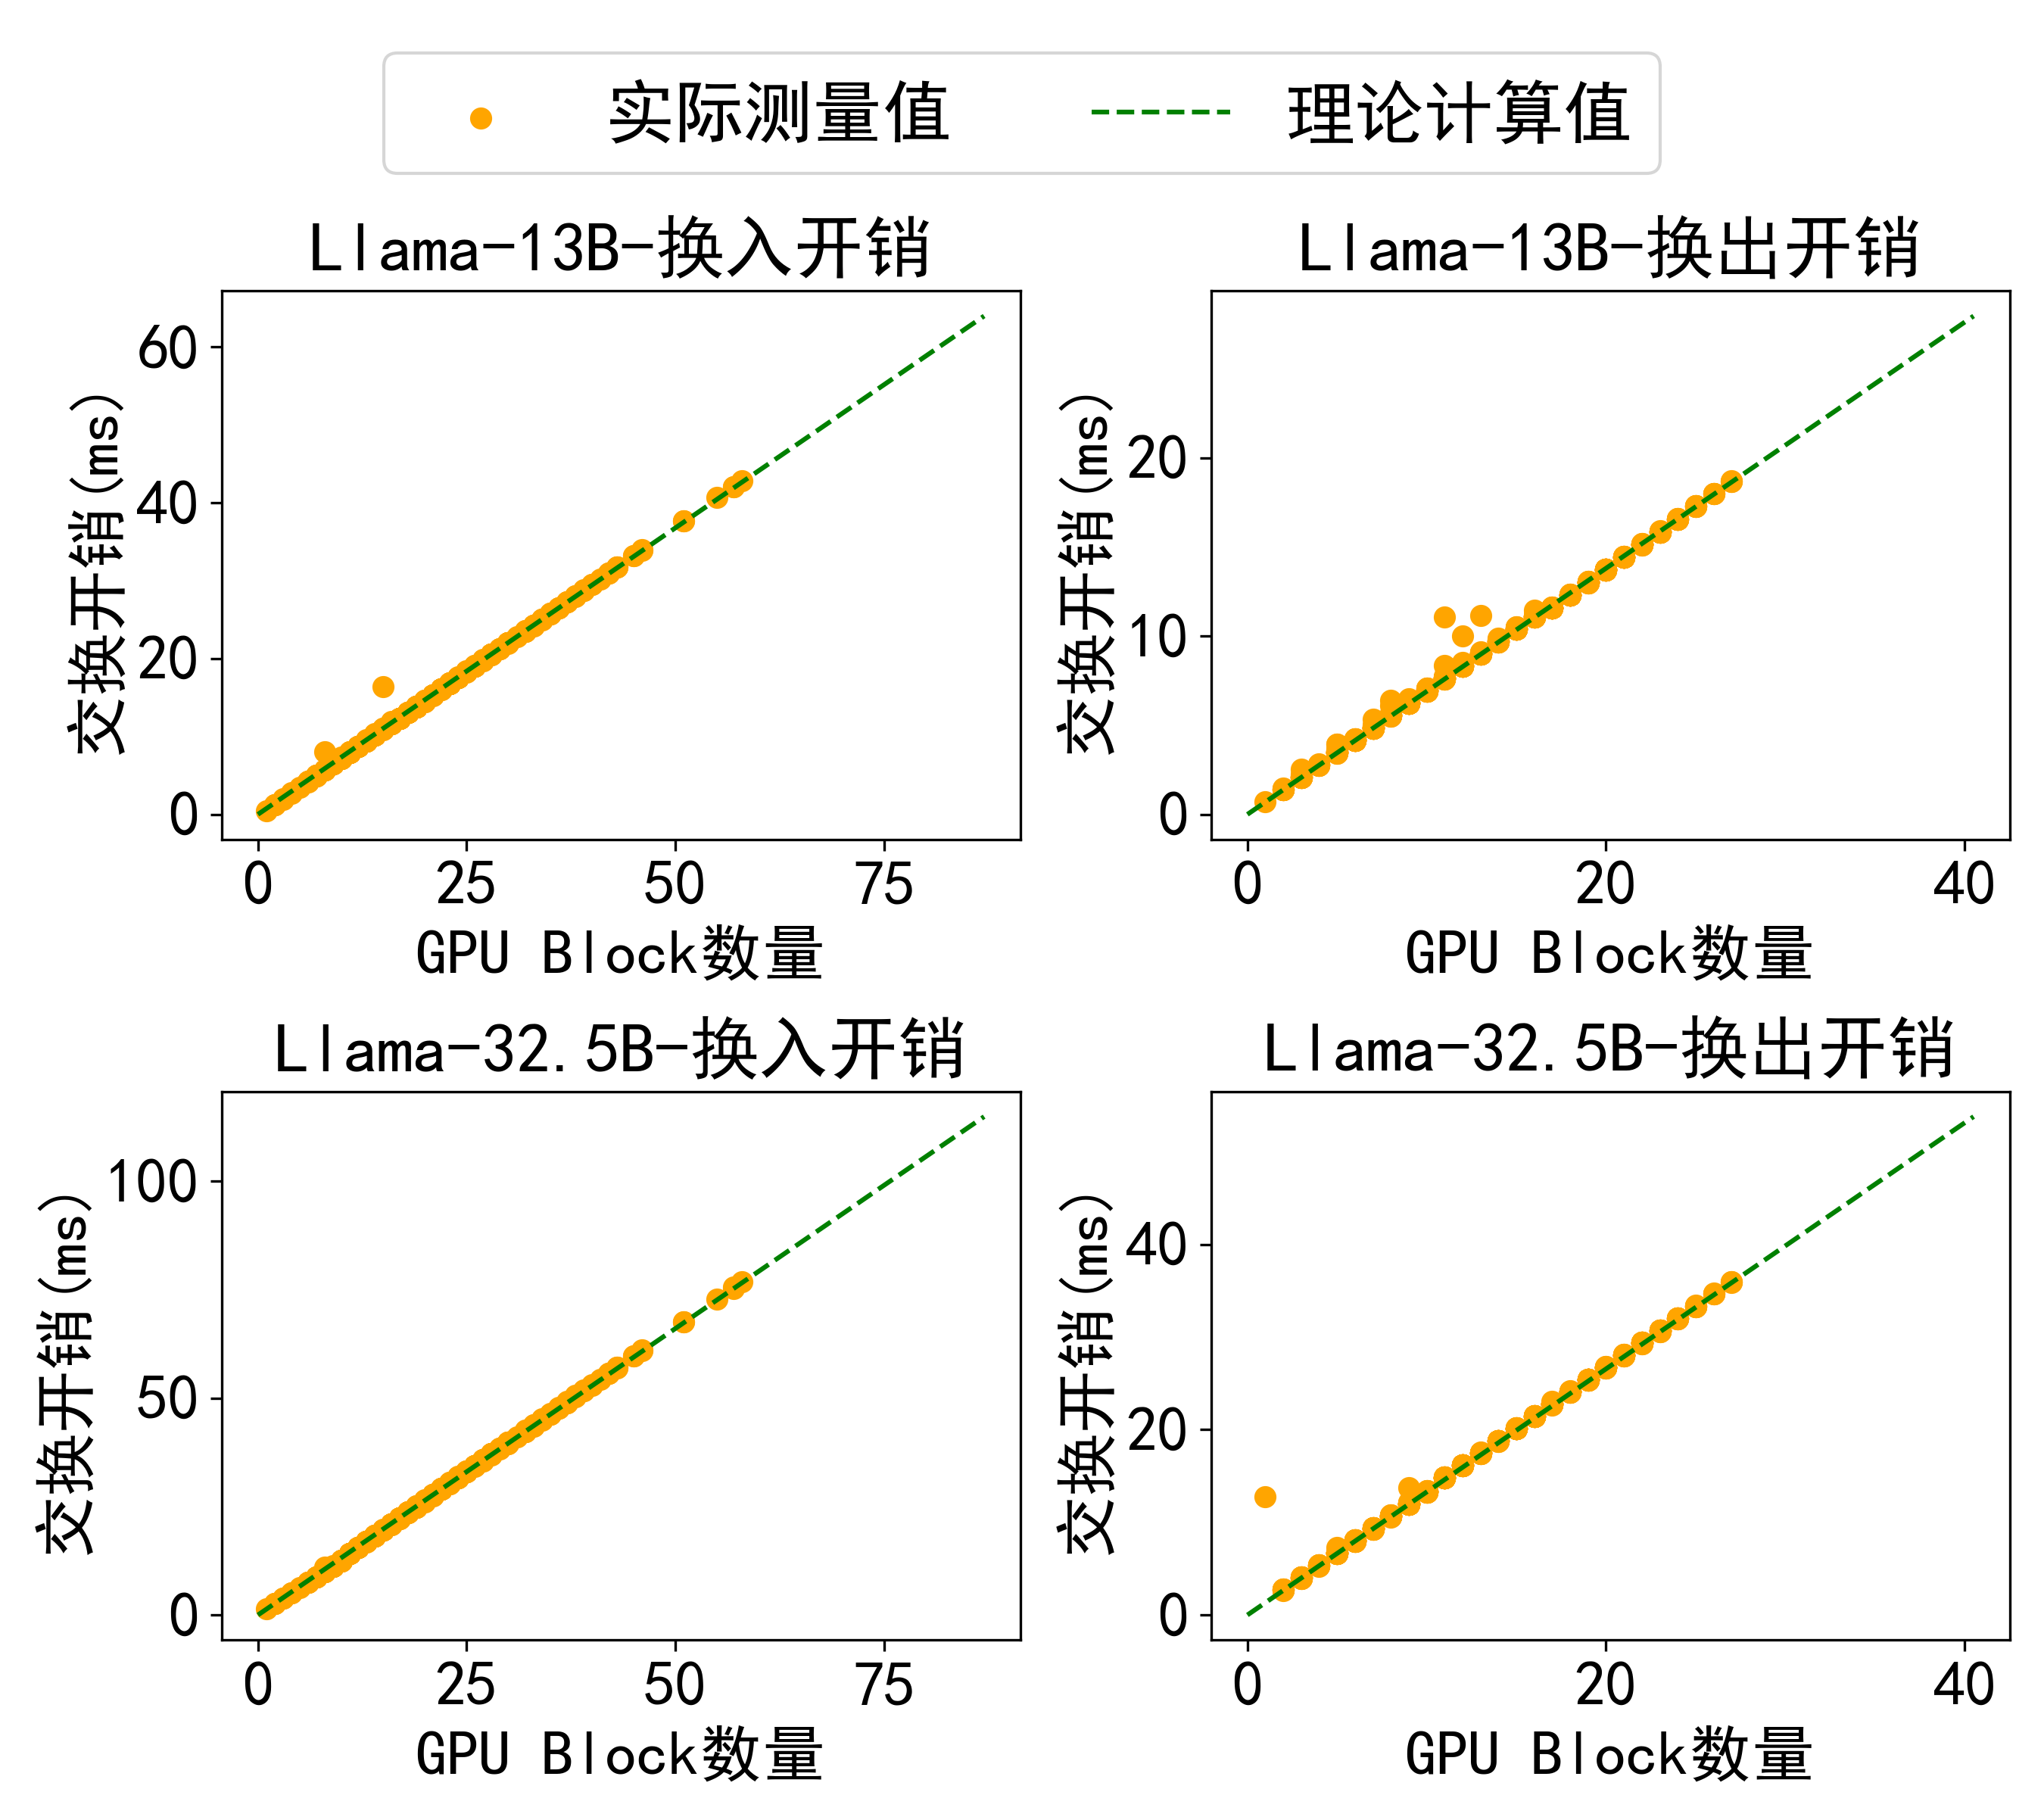
\includegraphics[width=0.90\linewidth]
  {交换开销预测误差.png}
  \caption{交换开销预测误差}
  \label{Fig:交换开销预测误差}
\end{figure}

张量重算(单次prefill阶段执行)开销的预测误差等于单步推理执行时间预测器的误差,根据本章第三节的分析可知,其预测误差低于2\%。 \par

本文针对模型Llama-13B和Llama-32.5B进行交换误差测试,其结果如图\ref{Fig:交换开销预测误差}所示。两个模型换入开销预测MAPE误差分别为1.5\%和1.1\%;换出开销预测MAPE误差分别为1.0\%和1.2\%。因此,张量交换开销总预测误差低于4\%。

\subsubsection{开销分析}

基于开销感知的内存优化策略在获取重算和交换开销时,会带来新的预测开销。本文设计如下对照实验获取张量感知过程的开销:  \par

在吞吐率测试过程中,当GPU内存不足时调用开销比较过程,但最终使用vLLM提供的固定式张量抢占策略(重算)。观察此情景下推理任务的总用时可知,张量感知过程的开销在整个推理任务中仅占0.1\%至1\%。


